% Masse kl: 4.4531 # in g (gegeben)
% Masse gr: 4.9528 # in g (gegeben)
% Durchmesser kl. Kugel: 1.5570+/-0.0010 (in cm)
% Durchmesser gr. Kugel: 1.5760+/-0.0010 (in cm)
% Volumen der kl. Kugel: 1.976+/-0.004 (in cm^3)
% Volumen der gr. Kugel: 2.050+/-0.004 (in cm^3)
% Dichte der kl. Kugel: 2.253+/-0.004 (in g/cm^3)
% Dichte der gr. Kugel: 2.416+/-0.005 (in g/cm^3)
% Gemittelte Fallzeit (hoch) kl: 12.20+/-0.13, gr: 34.75+/-0.16
% Gemittelte Fallzeit (runter) kl: 12.14+/-0.11, gr: 34.73+/-0.09
% Viskosität hoch: 1.170+/-0.013 (in mPa*s)
% Viskosität runter: 1.164+/-0.011 (in mPa*s)
% Apparatekonstante K_gr_h: 0.02374+/-0.00030 (in mPa*cm^3/g)
% Apparatekonstante K_gr_r: 0.02364+/-0.00025 (in mPa*cm^3/g)
% Reynoldsche Zahl Re_kl_h: 110.2+/-2.4
% Reynoldsche Zahl Re_kl_r: 111.3+/-2.0
% Reynoldsche Zahl Re_gr_h: 19.35+/-0.24
% Reynoldsche Zahl Re_gr_r: 19.46+/-0.19
%
% K_kl = 0.07640 (in m*Pa*cm^3/g) (gegeben)
% dichte_wasser = 0.998207 (in g/cm^3) (Internet)
% aus Plot:
% ln(A) = -5.567 ± 0.097
% B = 1680+/-30
% A = 0.0038+/-0.0004
%
\section{Auswertung}
\label{sec:Auswertung}
\subsection{Viskosität von Wasser bei Raumtemperatur}
\label{sec:Viskosität von Wasser}
Zunächst wird die Dichte der kleinen Glaskugel $\rho_{\text{kl}}$ durch die Gleichung 
(\ref{eqn:DichtefunktionKugel}) und Gleichung (\ref{eqn:VolumenKugel}) bestimmt. 
Dafür werden die gegebene Masse $m_{\text{kl}} = 4.4531\,\unit{\gram}$ und der 
gemessene Durchmesser $d_{\text{kl}}= \left(1.5570 \pm 0.0010\right)$ \unit{\centi \meter} 
verwendet.
$$\rho_{\text{kl}} = \left(2.253 \pm 0.004\right)\unit[per-mode=fraction]{\gram\per\cubic\centi\meter}$$ 
Die betrachteten Fallzeiten der kleinen Kugel sind in dieser Tabelle erfasst:
\begin{table}[H]
  \centering
  \caption{Gemessene Fallzeiten der kleinen Kugel bei einer Strecke von $10\, \unit{\centi\meter}$}
  \begin{tblr}{colspec={c c}}
      \toprule
      $t_{\text{Runter}}\, \left[\unit{\second}\right]$ & $t_{\text{Hoch}}\, \left[\unit{\second}\right]$ \\ 
      \midrule
      12.32 & 12.20\\
      12.18 & 12.35\\
      12.15 & 12.43\\
      12.24 & 12.23\\
      12.18 & 12.19\\
      12.18 & 12.26\\
      12.17 & 12.17\\
      11.92 & 12.10\\
      12.01 & 11.91\\
      12.07 & 12.19\\
      \bottomrule
  \end{tblr}
\end{table}
\noindent
Anhand dieser Messdaten erhält man die folgenden Zeiten, die für die Berechnung der Viskosität benötigt werden:
\begin{align*}
  t_{\text{kl,r}} &= \left(12.14\pm0.11\right)  \unit{\second}\\
  t_{\text{kl,h}} &= \left(12.20\pm0.13\right)  \unit{\second}\,.
\end{align*}
Die Viskosität von Wasser bei Raumtemperatur lässt sich mithilfe der Gleichung (\ref{eqn:EmpirischeEtaFunktion}) 
und der angegebenen Apparatekonstante der kleinen Glaskugel $K_{kl}= 0.0760 \,\unit[per-mode=fraction,inter-unit-product=\cdot]{\milli\pascal\cubic\centi\meter\per\gram}$
bestimmen.
\begin{align*}
  \eta_{\text{Hoch}} &= \left(1.170\pm0.013 \right) \unit[inter-unit-product=\cdot]{\milli\pascal\second}\\
  \eta_{\text{Runter}} &= \left(1.164\pm0.011 \right) \unit[inter-unit-product=\cdot]{\milli\pascal\second}
\end{align*}
%
\subsection{Apparatekonstante der großen Glaskugel}
\label{sec:Apparatekonstante der großen Glaskugel}
Vorab wird erneut mit der Gleichung (\ref{eqn:DichtefunktionKugel}) und der Gleichung (\ref{eqn:VolumenKugel})
die Dichte der großen Glaskugel bestimmt. Hierbei beträgt die gegebene Masse $m_{\text{gr}}= 4.9528 \;\unit{\gram}$ und 
der gemessene Durchmesser $d_{\text{gr}}=\left(1.5760\pm0.0010\right) \unit{\centi\meter}$.
$$\rho_{\text{gr}} = \left(2.416\pm0.005\right)\unit[per-mode=fraction]{\gram\per\cubic\centi\meter}$$ 
%
Die betrachteten Fallzeiten der großen Kugel sind in dieser Tabelle erfasst:

\begin{table}[H]
  \centering
  \caption{Gemessene Fallzeiten der großen Kugel bei einer Strecke von $5\,\unit{\centi\meter}$}
  \begin{tblr}{colspec={c c}}
      \toprule
      $t_{\text{Runter}}\, \left[\unit{\second}\right]$ & $t_{\text{Hoch}}\, \left[\unit{\second}\right]$ \\ 
      \midrule
      34.61 & 34.70 \\
      34.78 & 34.64 \\
      34.69 & 35.00 \\
      34.87 & 34.86 \\
      34.69 & 34.56 \\
      \bottomrule
  \end{tblr}
\end{table}
Aus den Messdaten werden die folgenden Zeiten bestimmt:
%
\begin{align*}
  t_{\text{gr,r}} &= \left( 34.73\pm0.09\right)  \unit{\second}\\
  t_{\text{gr,h}} &= \left(34.75\pm0.16 \right)  \unit{\second}\,.
\end{align*}
Folglich wird mit der Gleichung (\ref{eqn:KFunktion}) und den zuvor berechneten Viskositäten die 
Apparatekonstante der großen Glaskugel bestimmt.
\begin{align*}
  K_{\text{gr,r}} &= \left(0.02364\pm0.00025  \right)  \unit[per-mode=fraction,inter-unit-product=\cdot]{\milli\pascal\cubic\centi\meter\per\gram}\\
  K_{\text{gr,h}} &= \left(0.02374\pm0.00030  \right)  \unit[per-mode=fraction,inter-unit-product=\cdot]{\milli\pascal\cubic\centi\meter\per\gram}
\end{align*}
%
\subsection{Bestimmung der Reynoldschen Zahl}
Durch einsetzen der Werte in die Gleichung (\ref{eqn:Reynoldszahl}) ergeben sich für die 
kleine Glaskugel diese Reynoldszahlen:
\begin{align*}
  Re_{\text{kl,r}} &= \left(111.3\pm2.0\right)\\
  Re_{\text{kl,h}} &= \left(110.2\pm2.4\right).
\end{align*}
Analog erfogt die Berechnung der Reynoldszahlen für die große Glaskugel.
\begin{align*}
  Re_{\text{gr,r}} &= \left(19.46\pm0.19\right)\\
  Re_{\text{gr,h}} &= \left(19.35\pm0.24\right)
\end{align*}
Aus den Reynoldszahlen erschließt sich, dass sowohl bei der kleinen als auch bei der großen Glaskugel
eine laminare Strömung entsteht, da alle Reynoldzahlen deutlich kleiner sind als $Re=2000$.
%
\subsection{Temperaturabhängigkeit der Viskosität von Wasser}
Für die Auswertung der Temperaturabhängigkeit der Viskosität von Wasser wird der natürliche
Logarithmus von der Andradeschen Gleichung (\ref{eqn:AndradescheGleichung}) gebildet. Somit ensteht ein
linearer Zusammenhang zwischen dem Kehrwert von der Temperatur und dem natürlichen Logarithmus
von der dynamischen Viskosität $\eta$.
\begin{align}
  \begin{split}
   \eta (T) &= A \cdot e^{\frac{B}{T}}\\
    \Rightarrow \ln\left(\eta\left(T\right)\right) &= \ln \left(B\right) \cdot \frac{1}{T} + \ln\left(A\right)
    \label{eqn:lnEta}
  \end{split}
\end{align}
Die mithilfe von Gleichung (\ref{eqn:EmpirischeEtaFunktion}) gemessenen Fallzeiten der großen Kugel bei variierter Temperatur sind in der folgenden Tabelle
aufgeführt:
\begin{table}[H]
  \centering
  \caption{Gemessene Fallzeiten der großen Kugel bei unterschiedlichen Temperaturen}
  \begin{tblr}{colspec={c c c c c}}
      \toprule
      $T\, \left[\unit{\celsius}\right]$ & $t_{\text{h1}}\, \left[\unit{\second} \right]$ & $t_{\text{r1}}\, \left[\unit{\second} \right]$ & $t_{\text{h2}}\, \left[\unit{\second} \right]$ & $t_{\text{r2}}\, \left[\unit{\second} \right]$ & $\rho(T)\,\left[\unit[per-mode=fraction]{\gram\per\cubic\centi\meter} \right]$ (Q\cite{dichte})\\
      \midrule
      31\pm1 & 28.76 & 28.26 & 28.27 & 28.80 & 0.99534 \\
      33\pm1 & 27.16 & 27.03 & 27.12 & 27.07 & 0.99470 \\
      34\pm1 & 26.76 & 27.01 & 26.75 & 26.76 & 0.99437 \\ 
      36\pm1 & 26.16 & 26.06 & 26.16 & 26.24 & 0.99369 \\
      40\pm1 & 24.32 & 24.23 & 24.40 & 24.23 & 0.99222 \\
      42\pm1 & 23.52 & 23.46 & 23.36 & 23.49 & 0.99144 \\
      43\pm1 & 22.84 & 22.81 & 22.87 & 23.27 & 0.99104 \\
      44\pm1 & 22.38 & 22.64 & 22.23 & 21.80 & 0.99063 \\
      47\pm1 & 21.32 & 21.69 & 21.38 & 21.24 & 0.98936 \\
      49\pm1 & 20.64 & 20.81 & 20.58 & 20.41 & 0.98848 \\
      \bottomrule
  \end{tblr}
\end{table}
Im Abschnitt \ref{sec:Viskosität von Wasser} wurde bereits festgestellt, dass die dynamischen Viskositäten 
der beiden Fallrichtungen bei Raumtemperatur keine signifikante Differenz aufweisen. Aus diesem Grund werden
bei dieser Auswertung die Fallrichtungen \glqq hoch\grqq{} und \glqq runter\grqq{} nicht mehr getrennt voneinander
betrachtet. Demnach erhält man für die jeweiligen Temperaturen die folgenden Fallzeiten:
\begin{table}[H]
  \centering 
  \caption{Fallzeiten der großen Kugel und die temperaturabhängige Viskositäten}

  \begin{tblr}{colspec={c c c c}}
      \toprule
      $T\, \left[\unit{\celsius}\right]$ & $t\, \left[\unit{\second} \right]$ & $\rho(T)\,\left[\unit[per-mode=fraction]{\gram\per\cubic\centi\meter} \right]$ (Q\cite{dichte}) & $\eta\left(T\right)\, \left[ \unit[inter-unit-product=\cdot]{\milli\pascal\second}\right] $\\
      \midrule
      31\pm1 & 28.510 \pm 0.250 & 0.99534 & 0.962 \pm 0.014 \\
      33\pm1 & 27.095 \pm 0.065 & 0.99470 & 0.908 \pm 0.011 \\
      34\pm1 & 26.885 \pm 0.125 & 0.99437 & 0.907 \pm 0.012 \\  
      36\pm1 & 26.110 \pm 0.050 & 0.99369 & 0.882 \pm 0.011 \\
      40\pm1 & 24.275 \pm 0.045 & 0.99222 & 0.821 \pm 0.010 \\
      42\pm1 & 23.490 \pm 0.030 & 0.99144 & 0.795 \pm 0.010 \\
      43\pm1 & 22.825 \pm 0.015 & 0.99104 & 0.772 \pm 0.009 \\
      44\pm1 & 22.510 \pm 0.130 & 0.99063 & 0.762 \pm 0.010 \\
      47\pm1 & 21.505 \pm 0.185 & 0.98936 & 0.729 \pm 0.011 \\
      49\pm1 & 20.725 \pm 0.085 & 0.98848 & 0.703 \pm 0.009 \\
      \bottomrule
  \end{tblr}
\end{table}
Die in der Tabelle aufgelisteten dynamischen Viskositäten $\eta\left(T\right)$ erschließen sich aus der Gleichung (\ref{eqn:EmpirischeEtaFunktion}) 
und den temperaturabhängigen Dichten.
Mithilfe dieser Daten und der Gleichung (\ref{eqn:lnEta}) lassen sich die Messwerte sowie
deren Unsicherheiten graphisch darstellen. 
\begin{figure}[H]
  \centering
  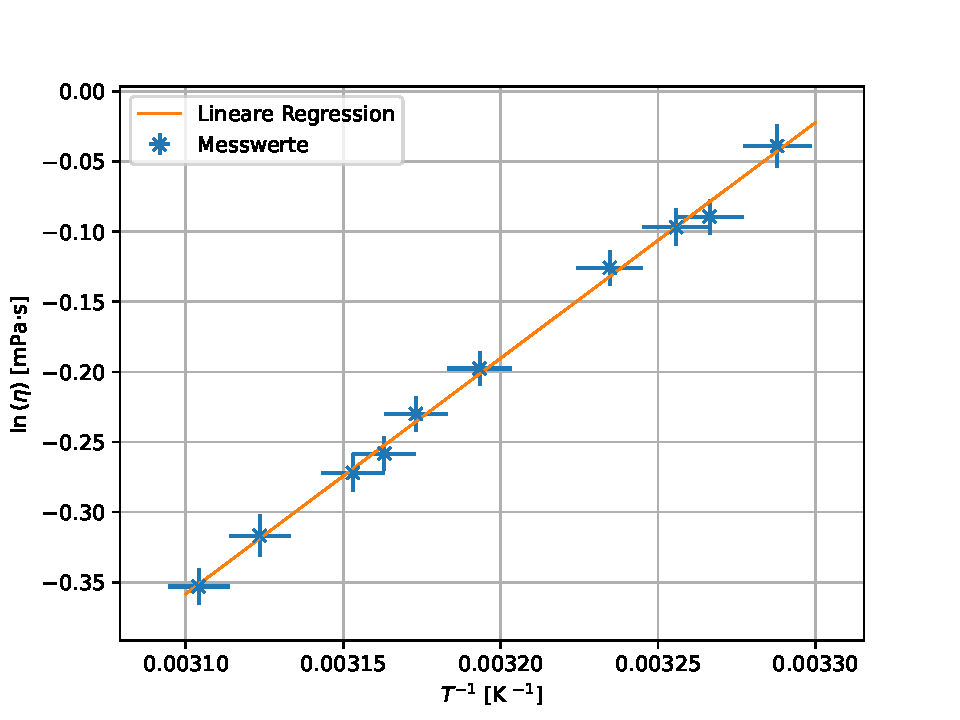
\includegraphics[width=0.92\textwidth]{plot.pdf}
  \caption{Lineare Ausgleichsgerade der Andradeschen Gleichung.}
  \label{fig:plot}
\end{figure}
Anschließend erfolgt die obige lineare Regression aus 
der Andradeschen Gleichung (\ref{eqn:AndradescheGleichung}). 
Anhand dieser linearen Regression und der Gleichung (\ref{eqn:lnEta}) werden die Konstanten $A$ und $B$ 
ermittelt. Hierbei entspricht $A$ dem Ordinatenabschnitt und $B$ der Steigung der 
linearen Ausgleichsgeraden.
\begin{align*}
  \ln\left(A\right) &= -5.567 \pm 0.097 \Longleftrightarrow A = 0.0038\pm0.0004\\
  B &= 1680\pm30
\end{align*}
%Siehe \autoref{fig:plot}!